\documentclass[12pt]{article}

\usepackage{pifont}
\usepackage{amsmath,amssymb}
\usepackage{siunitx}
\usepackage{geometry}
\usepackage{physics}
\usepackage{graphicx}
\usepackage{tikz}
\usepackage[utf8]{inputenc}
\usepackage{float}
\usepackage{enumitem}
\usepackage{hyperref} 
\hypersetup{
    colorlinks=true,
    linkcolor=blue,
    urlcolor=blue,
}
\usetikzlibrary{calc,decorations.pathreplacing,arrows.meta}
\geometry{a4paper, total={170mm,257mm}, left=20mm, top=20mm}

\begin{document}

\title{Projectile Motion Lab Report}
\author{Takumi Shiraishi}
\date{\today}
\maketitle

\tableofcontents
\vspace{1cm}


% ===================== SECTION: Muzzle Velocity ========================
\newpage
\section{Muzzle Velocity}
To determine theoretical range with projectile analysis, we find $v_i$ by muzzle velocity experiment. In this experiment, after Nikolay says 3, 2, 1, dart is launched from $1\mathrm{m}$ high and we are timing until hear the sound of dart hit the ground.
Five observers timed vertical launch at the same time to reduce individual reaction-time bias.

\subsection{Data Table (Vertical Time of Flight, s)}
Five observers measured the total vertical time of flight.

\begin{center}
\begin{tabular}{|c|c|c|c|c|}
\hline
Observer & Trial 1 (s) & Trial 2 (s) & Trial 3 (s) & Mean (s)\\ \hline
Takumi & 3.47 & 3.41 & 3.51 & 3.463 \\ \hline
Nikolay & 3.08 & 3.48 & 3.47 & 3.343 \\ \hline
Gursimran & 3.02 & 3.07 & 3.30 & 3.130 \\ \hline
Xander & 3.95 & 3.06 & 3.24 & 3.417 \\ \hline
Yiluo & 3.34 & 2.78 & 3.44 & 3.187 \\ \hline
\multicolumn{4}{|r|}{\textbf{Grand mean} $ t_{\mathrm{vert}}$} & \textbf{3.308} \\ \hline
\end{tabular}
\end{center}

% Image: muzzle_velocity.jpeg
\begin{figure}[H]
  \centering
  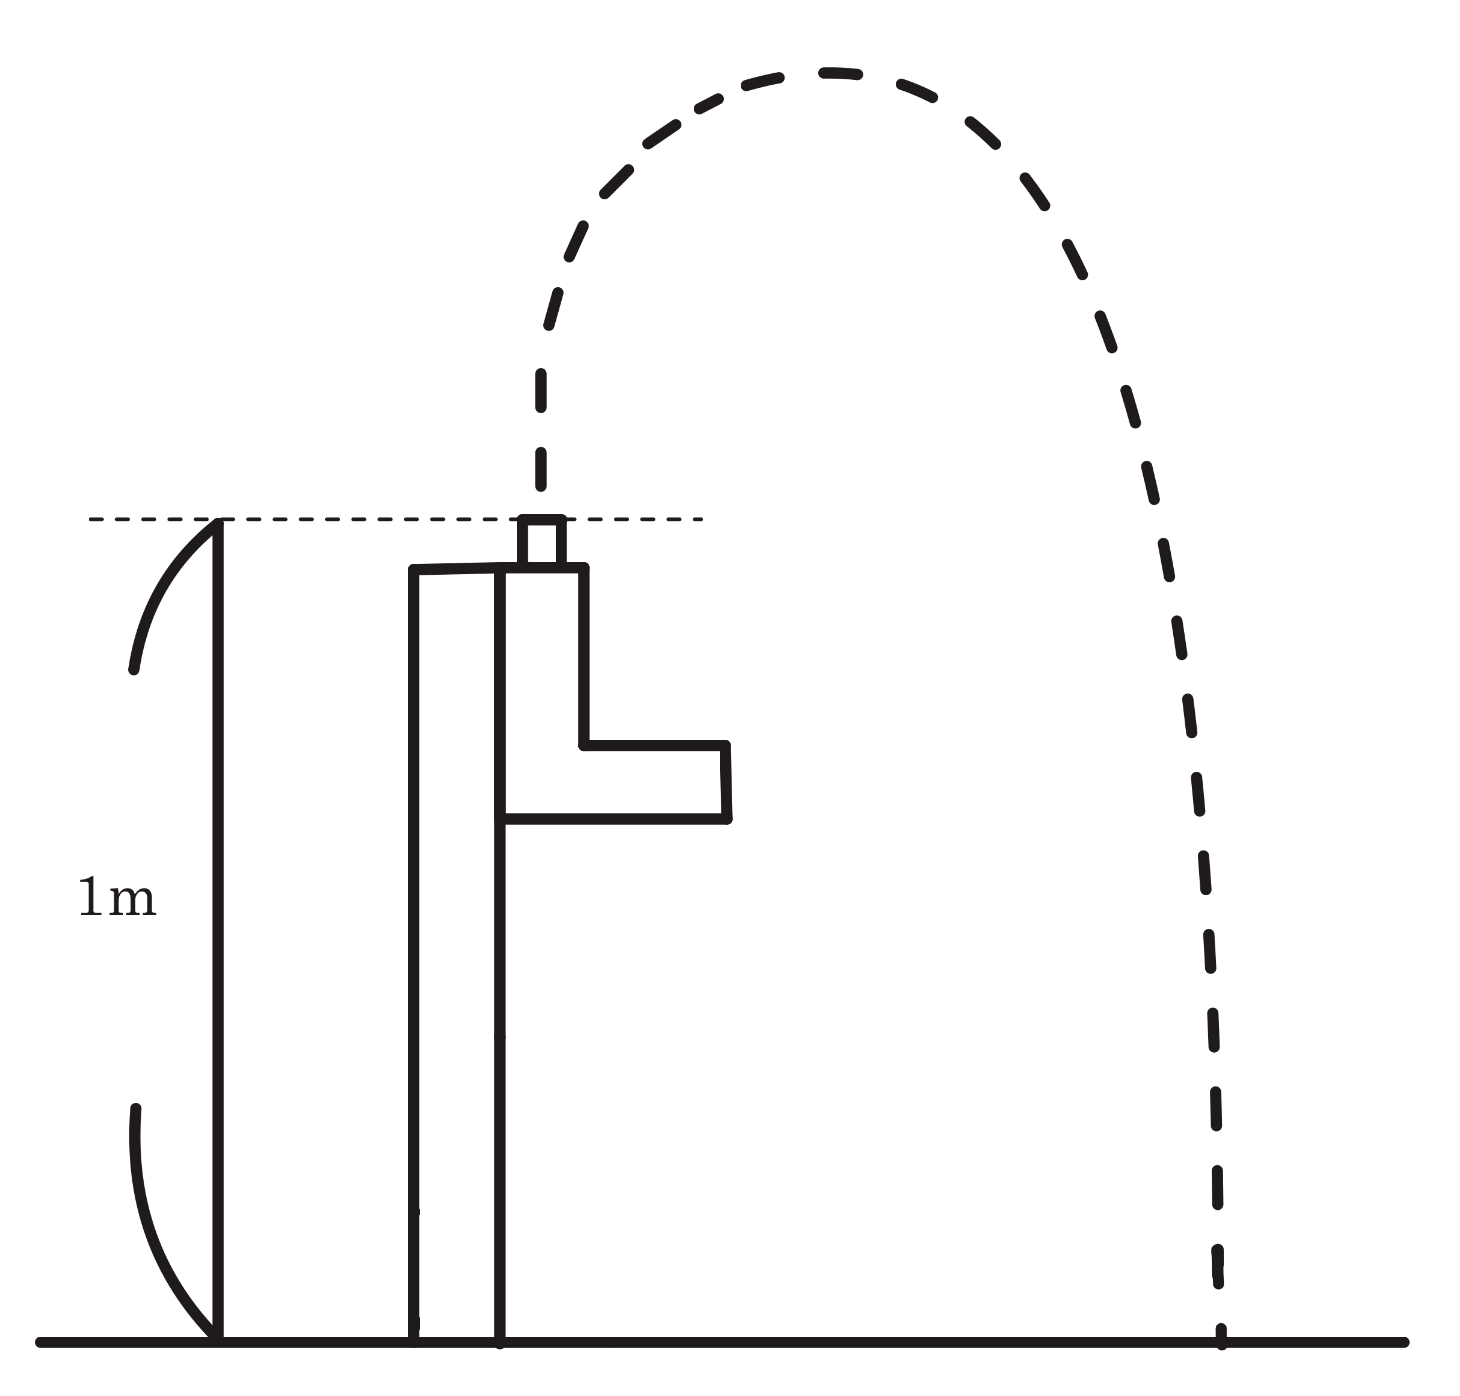
\includegraphics[width=0.85\linewidth]{muzzle_velocity.jpeg}
  \caption*{Diagram for vertical timing and Nerf Gun (aligned to the 1 m stick).}
\end{figure}

\subsection{Calculation to Find the Muzzle Velocity}
Take upward positive, so $a=-9.8~\mathrm{m/s^2}$ and $d=-1~\mathrm{m}$.
\[
d = v_i\, t + \tfrac{1}{2} a t^2 \quad \Rightarrow \quad
v_i = \frac{d - \tfrac{1}{2} a t^2}{t}.
\]
With $t=3.308~\mathrm{s}$:
\[
v_i = \frac{-1 - \tfrac{1}{2}(-9.8)(3.308)^2}{3.308}
= \frac{-1 + 4.9\,(3.308)^2}{3.308}
= \frac{-1 + 53.790}{3.308}
= \frac{52.790}{3.308}
\approx \boxed{15.96~\mathrm{m/s}}.
\]
\vspace{1em}

\noindent\hfill\underline{Initial velocity (Muzzle Velocity) of $15.96~\mathrm{m/s}$ upwards}

% ========================= SECTION: Range ==============================
\newpage
\section{Range}
By using Muzzle Velocity and projectile relation, it is possible to solve for theoretical range. In range experiment, the dart was launched horizontally from a height of $1~\mathrm{m}$ and the horizontal distances from five trials were averaged.

\subsection{Data Table (Experimental Range, m)}
\begin{center}
\begin{tabular}{|c|c|}
\hline
Trial & $R_{\exp}$ (m) \\ \hline
1 & 9.625 \\ \hline
2 & 9.862 \\ \hline
3 & 9.665 \\ \hline
4 & 9.695 \\ \hline
5 & 9.180 \\ \hline
\textbf{Average} & \textbf{9.605} \\ \hline
\end{tabular}
\end{center}

% Image: range.jpeg
\begin{figure}[H]
  \centering
  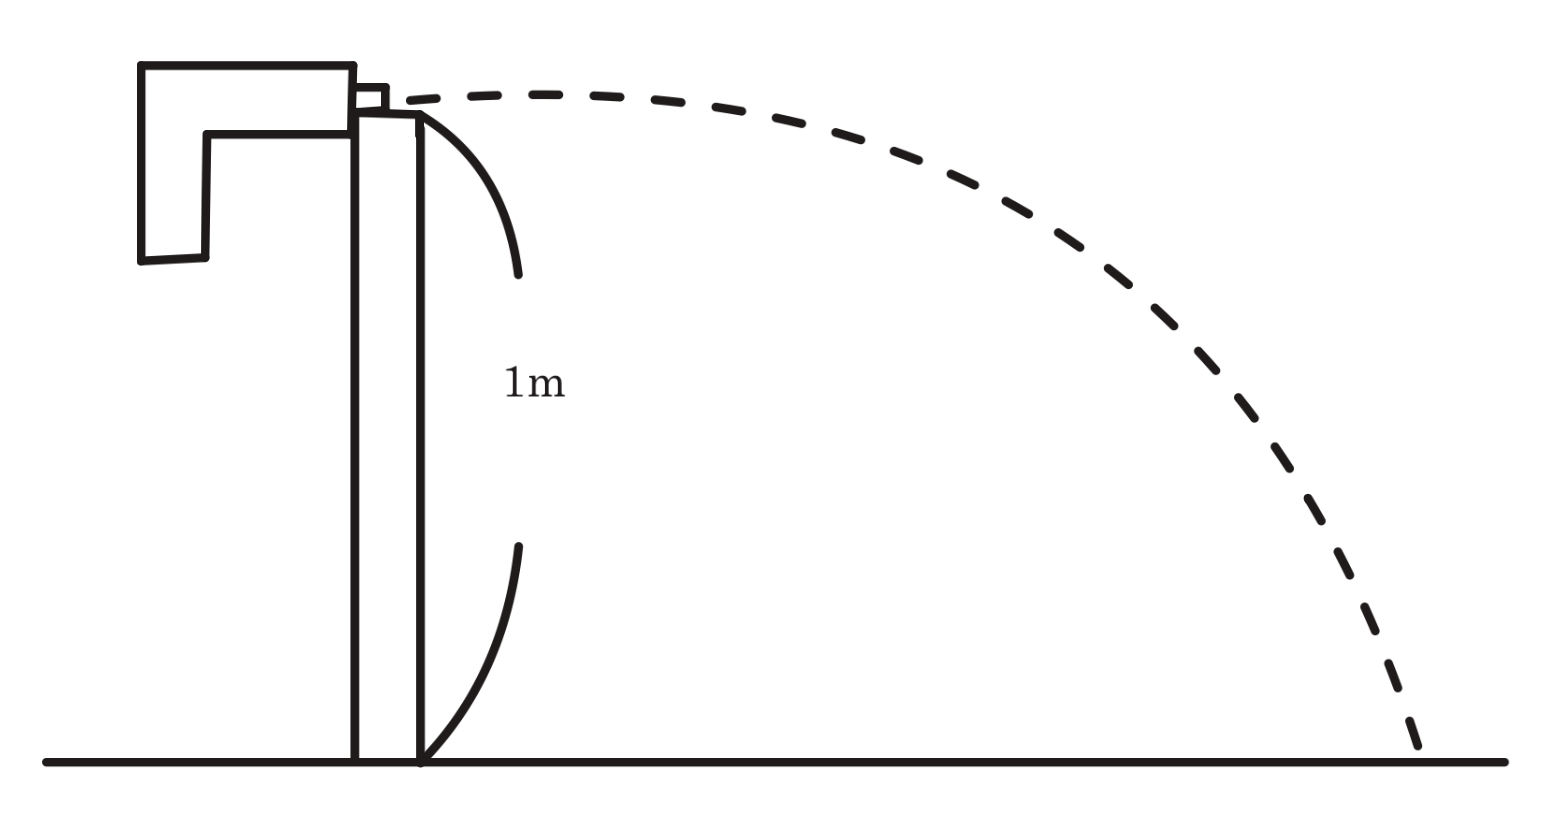
\includegraphics[width=0.85\linewidth]{range.jpeg}
  \caption*{Range measurement setup and marks.}
\end{figure}

\subsection{Calculation to Find Theoretical Range}
For a horizontal launch, the initial vertical speed is zero. The fall time is
\[
d = v_i t + \tfrac12 a t^2 \quad\Rightarrow\quad
t=\sqrt{\frac{2d}{a}}.
\]
With $a=-9.8~\mathrm{m/s^2}$ and $d=-1~\mathrm{m}$,
\[
t_{\mathrm{horiz}}
=\sqrt{\frac{2(-1)}{-9.8}}=0.4518~\mathrm{s}.
\]
Therefore,
\[
R_{\mathrm{theory}}=v_i\,t_{\mathrm{horiz}}
=(15.96)(0.4518)=\boxed{7.21~\mathrm{m}}.
\]

\vspace{1em}

\noindent\hfill\underline{Theoretical Range of $7.21~\mathrm{m}$}

% ========================= SECTION: Uncertainty ========================
\newpage
\section{Uncertainty}
\subsection{Muzzle Velocity Uncertainty}
\paragraph{(A) Timing and Muzzle Velocity}
In this report, we use a per–click reaction time of $t_r \approx 0.15~\mathrm{s}$ (auditory simple reaction time \cite{Kosinski2008}).
Because there are two clicks (start and stop),
\[
\Delta t_{\text{vert}} = 2\,t_r = 0.30~\mathrm{s}, \qquad t=3.308~\mathrm{s}.
\]

which gives
\[
\%\Delta t = \frac{\Delta t}{t} \times 100\%
= \frac{0.30}{3.308}\times 100\%\approx 9.07\%.
\]

Reported value:
\vspace{1em}
\[
\%\Delta t = 9.07\%
\]

\vspace{1em}


\paragraph{(B) Meter Stick and Muzzle Velocity}

Height of meter stick used during Muzzle Velocity experiment. The meter stick is aligned to the Nerf Gun; the dert extends $\pm 0.01~\mathrm{m}$. 
This $\pm 0.01~\mathrm{m}$ belongs to the vertical timing uncertainty, not to the Range experiment uncertainty.

We can calculate the displacement uncertainty as
\[
\%\Delta d=\frac{\Delta d}{d} \times 100\%=\frac{0.01}{1}\times 100\%=1\%
\]

Reported value: 
\[
\%\Delta d=1\%
\]

% Image: uncertainty.jpeg
\begin{figure}[H]
  \centering
  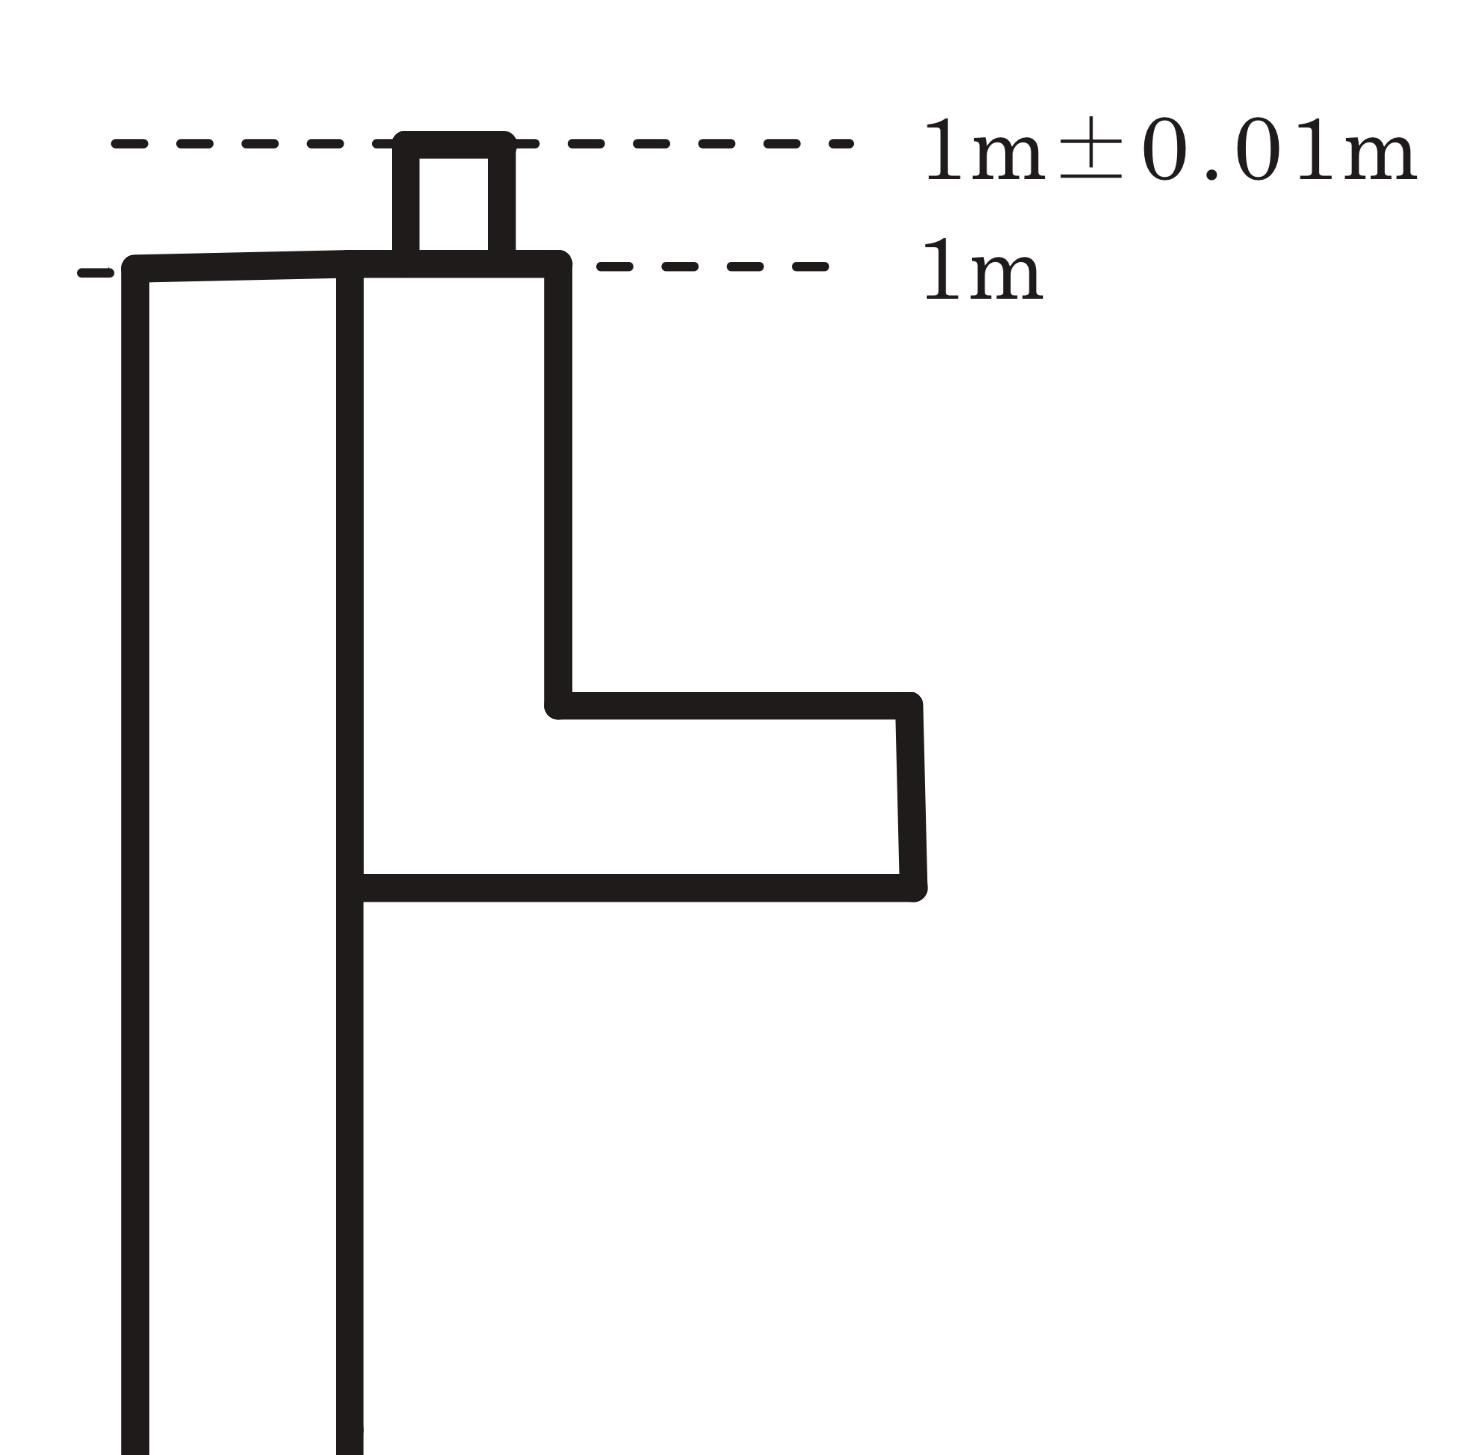
\includegraphics[width=0.60\linewidth]{uncertainty.jpeg}
  \caption*{Meter stick aligned; dart extends $\pm 0.01~\mathrm{m}$.}
\end{figure}

\paragraph{(C) Report Uncertainty}
To find the resultant Muzzle Velocity uncertainty, we use the kinematic relation
\[
d = v_i t + \tfrac12 a t^2 \quad\Rightarrow\quad
v_i = \frac{d - \tfrac12 a t^2}{t}.
\]

\vspace{1em}
As comparing Timing and Meter Stick uncertainty, 
Meter Stick uncertainty is much smaller than Timing uncertainty (1\% compared to 9.07\%). 
Therefore, we don't considerate displacement uncertainty. As well as constants.
\[
\Delta v_i \approx \frac{t^2}{t} \approx \Delta t
\]

which gives 
\[
\%\Delta v_i \approx \%\Delta t.
\]

Therefore, 
\[
\%\Delta v_i \approx 9.07\%.
\]
\vspace{1em}

However, I doubt myself about the part ``\emph{Meter Stick uncertainty is much smaller than Timing uncertainty}.''For justification (show $\%\Delta v_i \approx \%\Delta t$ in another way), I go back to the kinematic relation,

\[
d = v_i t + \tfrac12 a t^2 \quad\Rightarrow\quad
v_i = \frac{d - \tfrac12 a t^2}{t}.
\]

At $t=3.308~\mathrm{s}$
\[
\tfrac12 a t^2 = \tfrac12(-9.8)(3.308)^2 \approx -53.79~\mathrm{m},\qquad d=-1~\mathrm{m}.
\]
\vspace{1em}
So the numerator is
\[
d-\tfrac12 a t^2 = (-1)-(-53.79).
\]

The $-1~\mathrm{m}$ part is only about $1/53.79\approx 2\%$ of the gravity term. (Because we compare the magnitude between $d$ and $\tfrac12 a t^2$, we take absolute value)
\[
\frac{|d|}{\left|\tfrac{1}{2} a t^2\right|}
= \frac{1}{53.79}
\approx 0.0186 \; (\approx 2\%).
\]

For a $\%$uncertainty estimate we can ignore that small part and assume
\[
v_i \approx \frac{ \tfrac12(9.8)\,t^2 }{t} = 4.9\,t  \;\;\;\Rightarrow\;\; v_i \propto t.
\]

which I can justify
\[
\%\Delta v_i \approx  \%\Delta t \approx \boxed{9.07\%}.
\]

\vspace{1em}

\noindent\hfill\underline{Muzzle Velocity Uncertainty of $9.07\%$}


\subsection{Range Uncertainty}
\paragraph{(A) Experimental Range (meter sticks).}

\leavevmode \\[0.5em]

\textbf{Precision of Experimental Range:} 
From the data table, the standard deviation can be computed as
\[
\sigma=
\sqrt{\frac{\sum_{i}^{N}(x_i-x_{avg})^2}{N}}.
\]
$x_{avg}$ is
\[
x_{avg}=\frac{9.625+9.862+9.665+9.695+9.180}{5}\approx9.605.
\]
\vspace{1em}

Therefore,
\[
\sigma = 
\sqrt{\frac{\sum_{i}^{5}(x_i-9.605)^2}{5}}
\approx\boxed{0.227~\mathrm{m}}
\]

\vspace{1em}

It indicates that Experimental Range, $R_{exp}$ is precise. However, it does not mean it is accurate. We consider Range Readout and Dart Bounce as vital of uncertainty.
\vspace{1em}

\textbf{Range Readout and Experimental Range}
Initially, I assumed that whole measurement is tilted by a small angle $\theta$ compare to $R_{true}$:
\[
\cos\theta=\frac{R_{true}}{R_{means}}
\]

As isolate $R_{means}$,
\[
R_{means}=\frac{R_{true}}{\cos\theta}
\quad\Rightarrow\quad
R_{means}=R_{true}\cdot\sec\theta
\tag{1}
\]

\vspace{1em}

Difference between $R_{means}$ and $R_{true}$ can be expressed as
\[
\Delta R_{tilt} = R_{means} - R_{true}.
\]

Therefore,
\[
\%\Delta R_{tilt} = \frac{\Delta R_{tilt}} {R_{true}}\times 100\%=\frac{R_{means} - R_{true}}{R_{true}}\times 100\%
\tag{2}
\]

By (1) and (2),
\[
\%\Delta R_{tilt} = \frac{R_{true}\cdot\sec\theta - R_{true}}{R_{true}} \times 100\%= (\sec \theta - 1)\times 100\%.
\]

\vspace{1em}

However, $\%\Delta R_{tilt} = (\sec \theta - 1)\times 100\%$ applies only if whole meter sticks tilted by a specific angle $\theta$.

To generalize (applying for several meter stick stacking), we have to considerate increasing $\theta$ while stacking one more meter stick.
$N$ as number of meter sticks that fully used.
\[
\therefore \lfloor R_{means}\rfloor=N
\]

Meter stick is $1\mathrm{m}$ each, so $R_{true}$ can be expressed as
\[
R_{true}=1\cdot(\cos \theta+\cos 2\theta+\cdots \cos (\theta N))=\sum_{i=1}^{N} \cos\!\left(i\theta\right)
\tag{3}
\]

By (2) and (3),
\[
\%\Delta R_{tilt} = \frac{R_{means}-\sum_{i=1}^{N} \cos\!\left(i\theta\right)}{\sum_{i=1}^{N} \cos\!\left(i\theta\right)}\times 100\%
\]
\vspace{1em}

For a very careful setup with $\theta\le 5^\circ$,
\[
\%\Delta R_{tilt} = 
\frac{R_{means}-\sum_{i=1}^{N} \cos\!\left(5i^{\circ}\right)}{\sum_{i=1}^{N} \cos\!\left(5i^{\circ}\right)}\times 100\%.
\]
\vspace{1em}

Because we used 9 full meter sticks and read additional 0.61m ($R\approx 9.61~\mathrm{m}$), substitute $N=9$ and add $0.61\cos(10\cdot5^{\circ})$ to $R_{true}$.
\vspace{1em}
\[
\%\Delta R_{\text{tilt}} 
=
\frac{9.61-\sum_{i=1}^{9} \cos\!\left(5i^{\circ}\right)+0.61\cos(50^{\circ})}{\sum_{i=1}^{9} \cos\!\left(5i^{\circ}\right)+0.61\cos(50^{\circ})}\times 100\%.
\approx\boxed{15.18\%}.
\]
\vspace{1em}

Thus,
\[
\Delta R_{tilt} \approx 9.61 \cdot 0.1518 \approx 1.27 \ \mathrm{m} 
\]

\vspace{1em}

\textbf{Dart Bounce} when we measure for $R_{exp}$, the dart bounce off and go father than horizontal landing point. We assume bounce off is 0.20m,

\[
\Delta R_{bounce}=0.20~\mathrm{m} \ (\approx2.08\%).
\]

\vspace{1em}

\textbf{Experimental Range Uncertainty}
Experimental Range Uncertainty $\Delta R_{exp}$ can be computed as
\vspace{1em}
\[
\Delta R_{exp} \approx \Delta R_{tilt} + \Delta R_{bounce}.
\]

\vspace{1em}
From $\Delta R_{tilt}=1.27\mathrm{m}$ and $\Delta R_{bounce}=0.20\mathrm{m}$,
\[
\Delta R_{exp} \approx 1.27 + 0.20 = 1.47,
\]
Thus,
\[
\Delta R_{exp} \approx {9.61~\mathrm{m}~\pm~1.47~\mathrm{m}}
\]

\vspace{1em}

\noindent\hfill\underline{
Experimental Range of $9.61~\mathrm{m} \ \pm\ 1.47~\mathrm{m}\quad\text{}$
}

\paragraph{(B) Theoretical Range and Displacement (meter stick)}
For a horizontal launch,
\[
t_{\mathrm{horiz}}=\sqrt{\frac{2d}{a}},\qquad R_{\mathrm{theory}}=v_i\,t_{\mathrm{horiz}}.
\]

As $2$ and $a$ are constants in $\sqrt{\frac{2d}{a}}$,
\[
t \approx \sqrt{d} = d^{\frac{1}{2}}
\]

Therefore,
\[
\%\Delta t_{\mathrm{horiz}} \approx 
\tfrac12\%\Delta d 
= \tfrac12\,\frac{\Delta d}{d}\times 100
\]
\vspace{1em}


With a possible physically shaking, $d=1~\mathrm{m}\pm0.02~\mathrm{m}$,
\[
\%\Delta t_{\mathrm{horiz}} \approx \tfrac12\times\frac{0.02}{1}\times 100 = 1.00\%.
\]
Combine \% uncertainty by addition:
\[
\%\Delta R_{\mathrm{theory}} \approx \%\Delta v_i + \%\Delta t_{\mathrm{horiz}}
= 9.07\% + 1.00\% = \boxed{10.07\%}.
\]
Hence
\[
R_{\mathrm{theory}} = 7.21~\mathrm{m} \ \pm (10.07\%)
\;\approx\;
7.21~\mathrm{m} \pm 0.73~\mathrm{m}.
\]

\vspace{1em}


\noindent\hfill\underline{
Theoretical Range of 
$7.21~\mathrm{m} \pm 0.73~\mathrm{m}$
}

% ======== SECTION: Crank 3 Calculation & Reported Results =============
\newpage
\section{Crank 3 Calculation \& Reported Results}
\paragraph{Inputs and centers.}
Central values: $v_i=15.96~\mathrm{m/s}$, $d=-1~\mathrm{m}$, $a=-9.8~\mathrm{m/s^2}$.\\
Uncertainties: again, $\Delta t_{\text{vert}}=0.30~\mathrm{s}$ (from $t_r=150~\mathrm{ms}$) $\Rightarrow$
\[
\%\Delta v_i=\frac{0.30}{3.308}\times 100\%=9.07\%.
\]
Therefore, 
\[
v_i^{-}=15.96(1-0.0907)=14.51~\mathrm{m/s},\quad
v_i^{+}=15.96(1+0.0907)=17.41~\mathrm{m/s},
\]
and
\[
d^{-}=-1+0.02=-0.98~\mathrm{m},\qquad
d^{+}=-1-0.02=-1.02~\mathrm{m}.
\]

\paragraph{Base case.}
\[
t_0=\sqrt{\frac{2(-1)}{-9.8}}=0.4518~\mathrm{s},\qquad
R_0=v_i\,t_0=(15.96)(0.4518)=\boxed{7.21~\mathrm{m}}.
\]

\paragraph{Low (min) case.}
Use the smaller combination ($v_i^{-}=14.51~\mathrm{m/s}$, $d^{-}=-0.98~\mathrm{m}$):
\[
t^{-}=\sqrt{\frac{2(-0.98)}{-9.8}}=\sqrt{\frac{1.96}{9.8}}=0.4472~\mathrm{s},
\qquad
R_{\min}= (14.51)(0.4472)=\boxed{6.49~\mathrm{m}}.
\]

\paragraph{High (max) case.}
Use the larger combination ($v_i^{+}=17.41~\mathrm{m/s}$, $d^{+}=-1.02~\mathrm{m}$):
\[
t^{+}=\sqrt{\frac{2(-1.02)}{-9.8}}=\sqrt{\frac{2.04}{9.8}}=0.4563~\mathrm{s},
\qquad
R_{\max}= (17.41)(0.4563)=\boxed{7.94~\mathrm{m}}.
\]

\paragraph{Crank 3 report.}
Base and difference:
\[
R_{\text{theory}} = R_{0}\ \pm \  max(\ |R_0 - R_{min}| , \ |R_0 - R_{max}| \ )
= 7.21~\mathrm{m} \pm 0.73~\mathrm{m}
\quad(\%\Delta R_{theory} \approx 10.07\%.)
\]


% ======================= SECTION: Reported Results =====================
\newpage
\section{Reported Results}
\[
v_i = 15.96~\mathrm{m/s}\ \pm \ 
1.45~\mathrm{m/s}\ (\approx 9.07\%),
\quad
R_{\exp} = 9.61~\mathrm{m},
\quad
R_{\mathrm{theory}} = 7.21~\mathrm{m} \pm 0.73~\mathrm{m}\ (\approx 10.07\%).
\]
Percent difference:
\[
\text{Percent difference}=\frac{|Measured-Predicted|}{Predicted}\times 100\%=\frac{|9.61 - 7.21|}{7.21} \times 100\% \approx 33.3\% 
\]
\[
\Rightarrow \quad
\text{The experiment and theory do not agree within this uncertainty.}
\]

% ======================= SECTION: Conclusions =========================
\newpage
\section{Conclusions}
\begin{enumerate}[label=(\alph*), leftmargin=1.2cm]
  \item \textbf{You did two theoretical uncertainty estimations, one using proportional reasoning, the other using the crank 3 method. How to they compare, are they similar, do they differ? Explain why.} As a result, proportional reasoning and the Crank-3 method have approximately the same uncertainty ($\approx 10.07\%$). The similarity of these 2 methods because 
  \[
  R_{theory}=v_it_{horiz}, \quad t_{horiz}=\sqrt{\frac{2d}{a}}
  \]
  but also $2$, $a$ are constants,  $R_{theory} \propto v_i$. Therefore, this function act like linear. Proportional reasoning use linear approximation while crank 3 method calculate for actual min and max value. Linearity of the function made the similarity \cite{Taylor1997}.
  
  \item \textbf{Does your experimental (observable) data agree with the calculations using kinematic equations (theoretical). Consider your percent uncertainty from the initial instructions compared to your theoretical estimated uncertainties to help you explain “Why or Why Not” your experimental and theoretical values match?} $R_{\exp}=9.61~\mathrm{m}$ versus $R_{\mathrm{theory}}=7.21~\mathrm{m}\pm0.73~\mathrm{m}$ gives a percent difference of $33.3\%$, which is exceeded the uncertainty ($\%\Delta R_{theory}$). Likely air drag, underestimation of $v_i$, and setup alignment also make biases.
  For correction (find possible range that has $R_{exp}$), I assume that $R_{exp}$ is true (as it has low standard deviation) and predict that when Range Experiment, there were elevation of $\theta_{elevate}$.
    Use Kinematic Relation,
    \[
    d = v_i \sin \theta_{elevate} \cdot t_{horiz}+\tfrac12 at_{horiz}^2
    \]
    As $R_{exp}=9.61\mathrm{m}$,
    \[
    \begin{aligned}
    9.61 &= (15.96 \cos \theta_{elevate} )t_{horiz} \\
    t_{horiz} &= \frac{9.61}{15.96\cos\theta_{elevate}} \\
    \end{aligned}
    \]
    \vspace{1em}
    
    At $v_i=15.96~\mathrm{m/s}$ 
    $d=-1~\mathrm{m}$, $a=-9.8~\mathrm{m/s^2}$,
    \[
    \begin{aligned}
    -1 &= (15.96~\sin\theta_{elevate})t_{horiz} +\tfrac12(-9.8)t_{horiz}^2 \\
    \end{aligned}
    \]

    By $t_{horiz} = \frac{9.61} {15.96\cos\theta_{elevate}}$,
    \[
    \begin{aligned}
    -1 &= (15.96~\sin\theta_{elevate})\left(\frac{9.61} {15.96\cos\theta_{elevate}}\right) +\tfrac12(-9.8)\left(\frac{9.61} {15.96\cos\theta_{elevate}}\right)^2
    \end{aligned}
    \]
    \vspace{1em}
    Solve for $\theta_{elevate}$,
    \[
    \begin{aligned}
    \tan\theta&=\frac{9.61\pm\sqrt{9.61-4(1.78)(0.78)}}{2(1.78)} \\
    \theta &\approx 79.4^{\circ}, 4.7^{\circ}
    \end{aligned}
    \]

    \vspace{1em}

    Because I predict small elevation $\theta_{elevate}$, consider $4.7^{\circ}$. So there would be $4.7^{\circ}$ elevation to the horizontal when Range Experiment. This meets the uncertainty of 33.3 \%. 
    
  
\end{enumerate}

% ======================= SECTION: References ==========================
\newpage
\section{References and Resources}

The reference search was assisted by \emph{AI Research Assistant Elicit}, but all predictions, analysis, conclusions, etc. are my own.
\begin{thebibliography}{9}

\bibitem{Kosinski2008} 
Kosinski, R. J. (2008), ``A literature review on reaction time'', Clemson University. 

\bibitem{Taylor1997}
J. R. Taylor, \emph{An Introduction to Error Analysis}, 
2nd ed., University Science Books, 1997.

\end{thebibliography}


% ======================= SECTION: Code Repository ======================
\section*{Code Repository}
\vspace{0.5em}
The LaTeX source files and calculation snippets are available at:  
\url{https://github.com}

\end{document}
